\chapter{Analyse von artverwandten Spielen zur Konzeptentwicklung}\label{sec:analysis}

Das grundlegende Spielkonzept von \say{Connecting-Minds} wird durch die Analyse verwandter Spiele, wie sie im Kapitel \emph{\nameref{sec:sota}} beschrieben sind, sowie durch weitere Spiele mit vergleichbarem Spieldesign ergänzt. Ziel ist es, durch diese vergleichende Betrachtung Gestaltungsprinzipien und Mechaniken zu identifizieren, die als Inspiration und konzeptionelle Grundlage für die Entwicklung von \say{Connecting-Minds} dienen können.

Darüber hinaus sollen die Ergebnisse dieser Analyse zur Beantwortung der zentralen Forschungsfrage, \emph{\say{Welche spezifischen Eigenschaften muss eine solche Umgebung aufweisen und welche Kommunikationsparameter werden dabei angesprochen?}}, beitragen.

\section{Methodik}
Zur systematischen Analyse der artverwandten Spiele wurde ein mehrstufiges, eigens entwickeltes Analyseraster herangezogen. Dieses Raster gliedert sich in vier aufeinander aufbauende Abschnitte:

\subsection{Visuelle Analyse}
Im ersten Schritt wurde der Fokus auf die sichtbaren Rätsel- und Hinweiselemente innerhalb des visuellen Designs der untersuchten Spiele gelegt. Relevante Elemente wurde direkt im Bildmaterial markiert, um sie im Rahmen der nachfolgenden Auswertung gezielt untersuchen zu können. Diese Markierungen dienten der Identifikation wiederkehrender Gestaltungselemente sowie der Kategorisierung der eingesetzt Rätseldesigns. Darüber hinaus konnten auf diese Weise Interaktionsflüsse sichtbar gemacht und chronologisch geordnet werden. Zusätzlich wurden die jeweiligen Kamera- und Perspektivführungen sowie Ansichten auf die Spielumgebung berücksichtigt, um Rückschlüsse auf das räumliche Design ziehen zu können.

\subsection{Erstellung eines Diagramms zur Rätselstruktur}
Anschließend wurden für ausgewählte Spielabschnitte oder komplette Spielverläufe UML-Ablaufdiagramme erstellt. Ziel war es, die strukturelle Organisation sowie die logische Verknüpfung und Verschachtelung der Rätselinhalte zu erfassen. Die Vorgehensweise orientiert sich an methodischen Ansätzen zur Rätselstrukturierung, wie sie bspw. von \cite{tim_schafer_grim_1996} vorgeschlagen wurden.

\subsection{Deskriptive Übertragung}
Im dritten Schritt erfolgt eine deskriptive Zusammenführung der aus der visuellen Analyse und der strukturellen Diagrammerstellung gewonnenen Erkenntnisse. Diese wurden hinsichtlich ihrer Implikationen für das Design und die Gestaltung von Rätseln systematisch beschrieben.

\subsection{Schlussfolgerung}
Abschließend wurden die zuvor gewonnen Beobachtungen in Beziehung zur Konzeptentwicklung von Connecting-Minds gesetzt. Dabei wurde untersucht, welche Elemente potenziell übernommen, angepasst oder vermieden werden sollten, Diese Rückschlüsse flossen gezielt in die Weiterentwicklung der eigenen Konzepts ein.

\section{Auswahl der Stichprobe}
Die Auswahl der Spiele, die im Rahmen der Analyse näher untersucht wurden, erfolgt auf Grundlage spezifischer Kriterien und dient der gezielten Konzeptentwicklung für Connecting-Minds. Dabei wurden nicht sämtliche in Kapitel \ref{sec:sota} vorgestellten Spiele berücksichtigt. Ergänzend wurden weitere relevante Spiele in die Analyse einbezogen, die im vorherigen Kapitel nicht behandelt wurden, aber im Ergebnisabschnitt eingeführt und kontextualisiert werden.

Der Fokus der Analyse liegt auf Spielen, die über unterschiedliche Geräte oder Anwendungen hinweg gespielt werden müssen oder durch ihre asymmetrischen Rollen asymmetrische Interaktionen erzwingen. Aufgrund der konzeptionellen Ausrichtung von Connecting-Minds als asymmetrisches Multiplayer-Spiel wurde eine Auswahl getroffen, die besonders geeignete Beispiele für unterschiedliche Rollenverteilungen und Kommunikationsanforderungen im kooperativen Spielkontext liefert.

Konkret wurden die Spielreihe \say{We were here} sowie das Spiel \say{Myrmidon} als zentrale Analysekandidaten ausgewählt. Beide Titel bieten durch ihre Spielmechanik und das Rollenverständnis eine fundierte Grundlage für die Untersuchung asymmetrischer und kooperativer Multiplayerspiele. Ergänzt wird diese Auswahl durch das Indie-Adventure-Spiel \say{Tiny Room Stories: Town Mystery}, das, obwohl es ein Singleplayerspiel ist, durch seine strukturierte Rätselgestaltung Vorlagen für die Konzeption von Connecting-Minds liefert.

Von der Analyse ausgeschlossen wurden hingegen Spiele wie die Titel des Entwicklerstudios Hazelight, da deren Splitscreen-Mechanik es den Spielenden erlaubt, die Perspektive des Gegenübers unmittelbar nachzuvollziehen. Dadurch entfällt der Teil der Kommunikation zur Beschreibung des Spielgeschehens. Durch dieses zentrale Element in Connecting-Minds soll die Kommunikation provoziert werden. Ebenso wurde das Spiel \say{Keep Talking and Nobody Explodes} nicht in die engere Analyse aufgenommen, da hier lediglich eine Person aktiv im Spiel agiert, während die übrigen Teilnehmer außerhalb der Anwendung interagieren. Dieses Spielmodell wurde als nicht hinreichend relevant für die geplanten Designziele eingestuft und dient daher als Ausschlusskriterium. Das Spiel \say{The Past within} wurde ebenso aus dem Analysekreis ausgeschlossen, da dessen struktureller Aufbau nicht mit der angestrebten Weiterentwicklung von Connecting-Minds vereinbar war. In \say{The Past within} lösen die Spieler zunächst unabhängig voneinander Rätsel innerhalb ihrer eigenen Anwendung. Erst an bestimmten Punkten greift das Spielgeschehen ineinander, sodass eine kooperative Abstimmung notwendig wird. Diese Gestaltung führt jedoch dazu, dass der Bedarf an kontinuierlicher Kommunikation nur punktuell entsteht, da zunächst jeweils überprüft werden muss, ob die Unterstützung des Mitspielers überhaupt erforderlich ist.

\section{Ergebnisse der Analysen}

Im nächsten Schritt werden die ausgewählten Spiele \say{We were here}, \say{We were here too}, \say{Tiny Room Stories} und \say{Myrmidon} hinsichtlich ihrer relevanten Merkmale analysiert. Die Analyse erfolgt nach dem zuvor vorgestellten Schema und beleuchtet insbesondere die Darstellungen im Spiel, sowie die Rätselmechaniken und die daraus resultierenden kommunikativen Aspekte.

\subsection{We were here - Spielreihe}
In der vorliegenden Analyse wurde der Fokus auf die ersten beiden Teile der Spielreihe, \say{We were here} und \say{We were here too}, beschränkt. Eine umfassende Untersuchung aller Titel der Reihe hätte den Rahmen dieser Arbeit überschritten, während der zusätzliche Erkenntnisgewinn im Verhältnis zum Aufwand als gering einzuschätzen ist. Die ausgewählten Spiele wurden daher in erste Linie in der Breite untersucht und nicht der Menge, um grundlegende Strukturen der Interaktion und Kommunikation zu erfassen. Im Folgenden werden die beiden Titel gemeinsam betracht und als eine zusammengehörige Einheit analysiert.

\paragraph{Visuelle Analyse}
Die Abbildungen im Anhang \ref{sec:append_anylsis_wwh_wwht_visual}: \nameref{sec:append_anylsis_wwh_wwht_visual} geben einen Einblick in die Analyse der Spielerrollen in den beiden Spielen. Auffällig ist, dass die Rätselelemente überwiegend durch visuelle Elemente umgesetzt sind. Es müssen Symbole und bildhafte Darstellungen korrekt identifiziert und zugeordnet oder in einer bestimmten weise platziert werden. Die Rätsel sind dabei integraler Bestandteil der Spielwelt. Hinweise erscheinen entweder als Symbole an Wänden oder als in die Umgebung eingebettete Textelemente. Nur in der Ausnahmefällen erfolgt die Vermittlung der zu Lösung nötigen Informationen über auditive Elemente oder Texte in Büchern.

In \say{We were here} zeigt sich eine klare Rollenverteilung zwischen dem \say{Explorer}, der innerhalb der Spielwelt agiert und direkt mit den Rätseln konfrontiert ist, und dem \say{Librarian}, der sich in einem zentralen Hub aufhält, in dem er über die notwendigen Informationen zu den Lösungen verfügt. Der Spielfortschritt ist demnach auf eine enge zielgerichtete Kommunikation zwischen den beiden Rollen angewiesen. Ein ähnliches Muster zeigt sich in  \say{We were here too}. Der \say{Peasant} befindet sich dabei zunächst in rätselhaften Gewölben, während der \say{Lord} die korrespondierenden Informationen erhält und ebenfalls in rätselhaften Gewölben feststeckt. Im Vergleich zum ersten Teil wird letzterer jedoch häufiger aktiv in das Lösen von Rätseln eingebunden und bewegt sich ebenfalls durch verschiedene Räume, anstatt dauerhaft in einem zentralen Hub zu verbleiben.

\paragraph{Analyse des Rätseldesigns}
Die Abbildung im Anhang \ref{sec:append_riddles_wwh_wwht}: \nameref{sec:append_riddles_wwh_wwht} zeigen die Ablaufdiagramme der beiden Spiele \say{We were here} und \say{We were here too}. Auffällig ist, dass im ersten Teil die Rolle des \say{Librarian} im Kontext des Rätseldesigns einem weitgehend linearen Verlauf folgt. Verschachtelte oder mehrstufige Rätselstrukturen treten nur selten auf. Die Spielstruktur sieht in der Regel vor, dass der \say{Explorer} mit den eigentlichen Rätseln und Hindernissen in der Spielwelt konfrontiert wird, während der \say{Librarian} außerhalb dieser Räume agiert und die benötigten Informationen zur Lösung bereitstellt. Die Interaktion zwischen den Rollen ist dadurch überwiegend eindimensional und von einer klaren Aufgabenverteilung geprägt.

Im Nachfolger \say{We were here too} lassen sich im Vergleich vermehrt verschachtelte oder verkettete Rätselstrukturen erkennen, etwa in Raum zwei des Spiels. Solche komplexeren Designs bleiben jedoch die Ausnahme. Insgesamt wiederholt sich ein ähnlicher Aufbau wie im Vorgängerspiel. Die Rollenverteilung bleibt asymmetrisch, die Zusammenarbeit erfolgt primär über Informationsaustausch, und die Kommunikationsstruktur folgt weiterhin einem einfachen Muster aus Anfrage und Antwort.

\paragraph{Schlussfolgerung}
Der zentrale Aspekt der Kommunikationsaufforderung ist in beiden Spielen erkennbar. Er bildet eine gemeinsame Grundlage. In \say{We were here} fällt jedoch auf, dass das Rätseldesign häufig monoton und eindimensional wirkt. Der \say{Explorer} stößt auf Rätsel, beschreibt gegebene und/oder gesuchte Gegenstände, der \say{Librarian} geht in bestimmten Raum und beschreibt gesuchte Gegenstände, der \say{Explorer} löst Rätsel. Es existieren zwar einzelne Ausnahmen, in denen der \say{Librarian} aktiv werden muss um dem \say{Explorer} weiterzuhelfen, etwa als der\say{Librarian} das richtige Ventil vom Rohr öffnen musste. Doch diese wechselseitige Abhängigkeit bleibt die Ausnahme. Gerade diese Form der Verzweigung ist für \say{Connecting-Minds} essenziell und sollte eine tragende Rolle Spielen. Auf dieser Grundidee lässt sich aufbauen, auch wenn nicht jedes Rätsel in seiner konkreten Ausgestaltung überzeugt, bieten bestimmte Ansätze dennoch wertvolle Anregungen, besonders im Hinblick auf die Möglichkeit, abwechslungsreiche, variantenreichere und stärker auf Kooperation ausgelegte Rätsel für \say{Connecting-Minds} zu entwickeln.

Deutlich weiter geht das zweite Spiel, \say{We were here too}, in dem die gegenseitige Verflechtung zwischen den beiden Rollen wesentlich häufiger zum Tragen kommt. In vielen Fällen ist es der \say{Peasant}, der nicht nur seinen eigenen Weg zum nächsten Raum freischaltet, sondern zugleich auch den vom \say{Lord}. In zwei Fällen ist das Prinzip sogar umgekehrt gestaltet. Der \say{Lord} ermöglicht dem \say{Peasant} den Zugang zu neuen Bereichen. In einem der beiden Fällen muss der \say{Peasant} eine Wendeltreppe hinaufrennen, unter der sich der Boden langsam einzieht. Er kommt jedoch nur bis zu einer Speerwand, die über einen Würfel geöffnet werden kann. Er muss dem \say{Lord} den Aufschnitt des Würfels beschreiben, welcher den richtigen Würfel auswählen und in die Zielablage ablegen muss. Durch die Verschachtlung wird der Grundgedanke der Kommunikation und Zusammenarbeit deutlich verstärkt hervorgehoben und erzeugt ausgeglichenen Spaß in den Anwendungen. Ein weiterer Zusatz des Rätseldesigns ist das aufeinander Aufbauen von Rätseln. Dieses Element wird im Rahmen dieser Schlussfolgerung als \say{Mehrstufigkeit} bezeichnet und ist zum Beispiel in Raum zwei zu finden, bei dem aneinander gekettet, verschiedene Rätsel gelöst werden müssen.

Diese strukturelle Ausrichtung eignet sich grundsätzlich gut als gestalterische Vorlage, sofern sie sich sinnvoll in \say{Connecting-Minds} übertragen lässt. Gleichzeitig zielt \say{Connecting-Minds} auf eine noch tiefere und kontinuierliche Abhängigkeit zwischen den beiden Spielerrollen. Beide Rollen sollen nicht nur gelegentlich, sondern regelmäßig und systematisch aufeinander angewiesen sein. Die Zusammenarbeit wird damit zur unverzichtbaren Grundlage des Spielfortschritts. Aus der engen Verflechtung ergibt sich, dass Kooperation nicht nur hilfreich, sondern spielentscheidend wird.

Konzepte wie mehrstufige Rätsel oder Einsatz von zeitlichen Begrenzungen (Timer) sind in diesem Zusammenhang ebenfalls interessante Überlegungen. Während Mehrstufigkeit sich als zentrales Element für die Rätselgestaltung anbietet, sollte der Timer gezielt und situationsabhängig eingesetzt werden, da sein Einfluss stark vom jeweiligen Spannungsbogen und dem beabsichtigten Spielerlebnis abhängt.

\subsection{Tiny Room Stories: Town Mystery}
\say{Tiny Room Stories: Town Mystery} ist ein Escape-Room-Spiel mit eingebetteter Detektivgeschichte, für mobile Endgeräte (IOS und Android) sowie für den PC verfügbar. Die Spieler übernehmen die Rolle eines Privatdetektivs, der einen Hilferuf seine Vaters folgt und in die scheinbar verlassene seines Vaters reist. Ziel ist es, das Verschwinden der Einwohner aufzuklären, indem verschiedene Orte in der Stadt untersucht, Hinweise gesammelt, Rätsel gelöst und mechanische wie logische Sperren überwunden werden. 
Das Spiel verbindet Elemente vom Escape-Room-Design mit Merkmalen von Point-and-Click-Adventures. Eine Besonderheit stellt die vollständig drehbare \ac{3D}-Umgebung dar, die es den Spielern erlaubt, die einzelnen Level aus unterschiedlichen Perspektiven zu betrachten und so versteckte Hinweise oder interaktive Objekte gezielt aufzuspüren (vgl. \citealp{kiary_games_tiny_2021}).

Im Gegensatz zur \say{We were here}-Reihe handelt es sich bei \say{Tiny Room Stories: Town Mystery} um ein reines Singleplayerspiel. Der Fortschritt des Spiels erfolgt durch das Freischalten von Abschnitten und narrativen Informationen, wodurch die Handlung schrittweise aufgedeckt wird. Für die Analyse wurden der Prolog sowie Kapitel 1 des Spiels betrachtet. Der grundlegende Aufbau bleicht auch in den folgenden Kapiteln erhalten. Veränderungen ergeben sich primär in der inhaltlichen Gestaltung sowie in der Komplexität und Verschachtelung der jeweiligen Rätsel und Hinweise.

\paragraph{Visuelle Analyse}
Das in Anhang \ref{sec:append_analysis_trstm}: \nameref{sec:append_analysis_trstm} dargestellte Ergebnis gibt einen Überblick über die erste Analyse des Spiels. Der Schwerpunkt liegt dabei zunächst auf den Informationen und Anweisungen die das Spiel dem Spieler zu Verfügung stellt. Darauf aufbauend erfolgt eine Kategorisierung der Rätseltypen sowie eine Betrachtung der jeweiligen Lösungsmechanismen. Ergänzend wurde auf die Art und Darstellung von Steuerungshinweisungen geachtet, um potenzielle Übertragungsmöglichkeiten für die Konzeptentwicklung von \say{Connecting-Minds} zu identifizieren. Das Spiel zeichnet sich insgesamt durch die Spielumgebung eingebetteter Rätsel und kontextuelle Hinweise aus. Diese werden durch Notizzettel und andere schriftliche Verweise ergänzt, die das narrative Rätseldesign unterstreichen. Beide Designansätze greifen ineinander und ermöglichen ein abwechslungsreiches sowie mitunter herausforderndes Spielerlebnis.

\paragraph{Analyse des Rätseldesigns}
Abbildung \ref{fig:trs-uml} zeigt das Ablaufdiagramm der Rätsel des Spiels. Sowohl in der visuellen Darstellung des Spiels, als auch im Design der Rätsel ist erkennbar, dass Zugänge zu neuen Räumen neue Hinweise oder Rätsel freischalten, welche gelöst werden müssen. Die Rätsel sind dabei gegenseitig verwoben, sodass es oft vorkommt, dass das Lösen von Rätsel A erst Hinweise für Rätsel B zugänglich macht wodurch Rätsel C ebenso gelöst werden kann. Diese Struktur findet sich in Kapitel 1 beim Bücherregal Rätsel wieder, als auch bereits im Prolog beim Öffnen der Schranke.

\begin{figure}[ht]
\centering
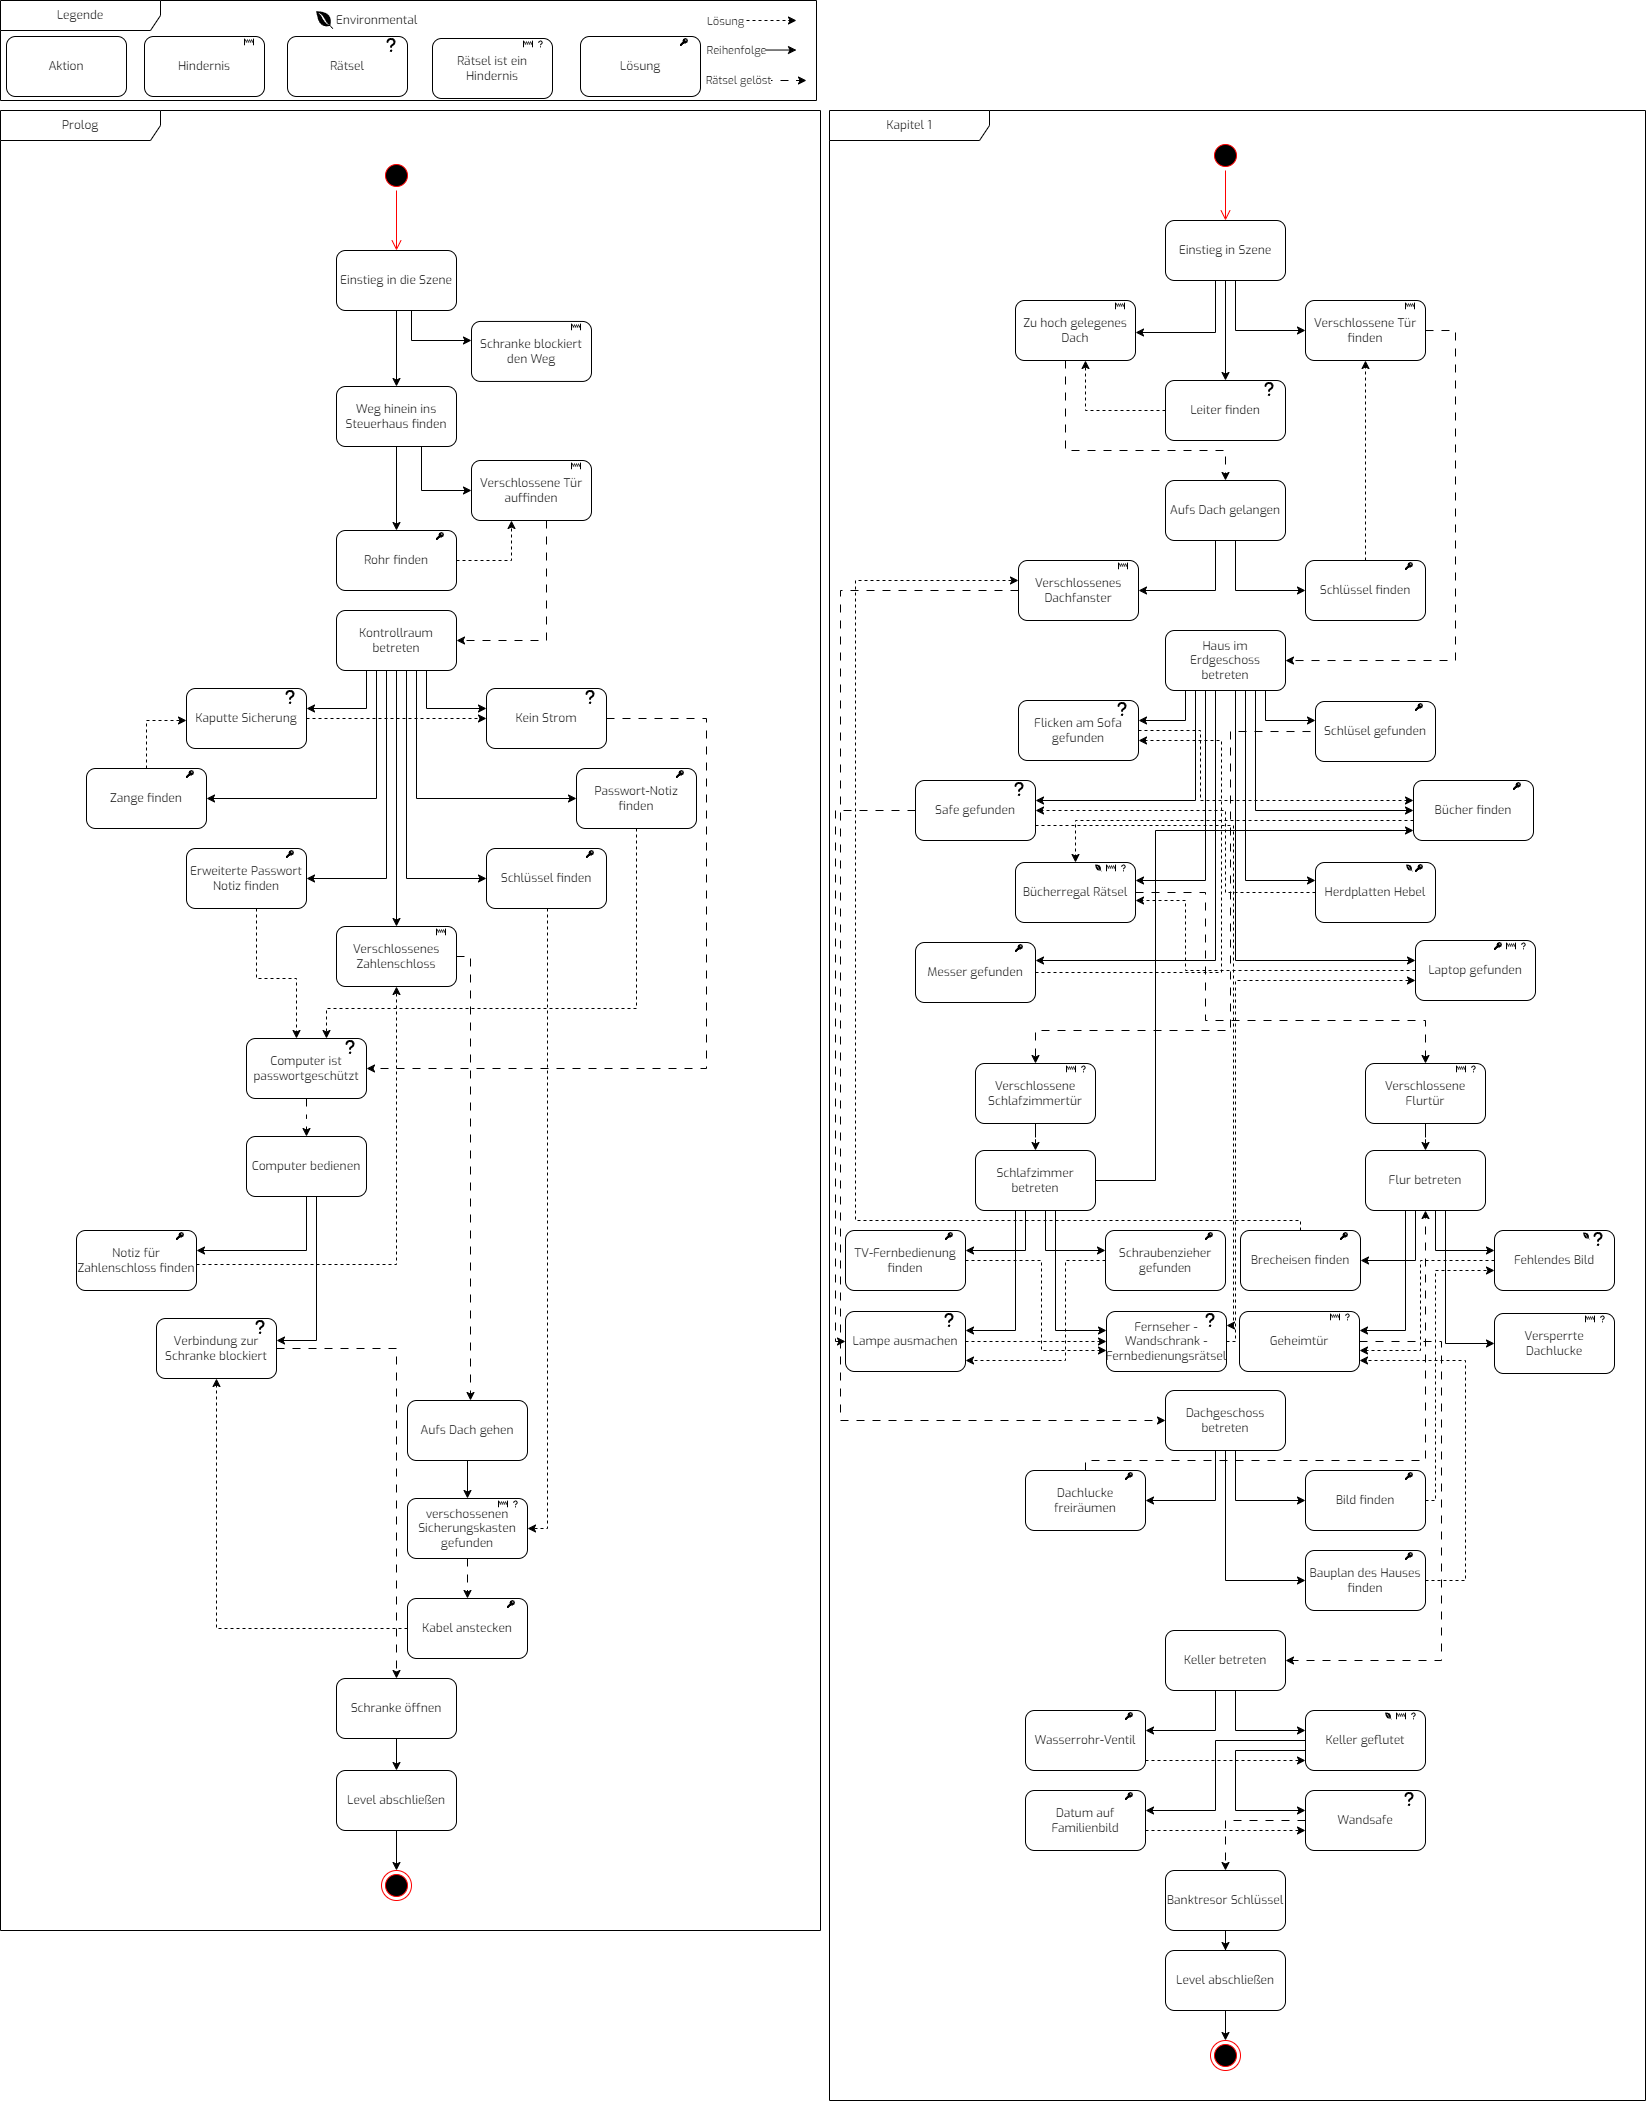
\includegraphics[width=1\linewidth]{content/pictures/TinyRoomStoriesUML.png}
\caption{Rätseldesign von Tiny Room Stories (Quelle: eigene Darstellung), vollständig in Anhang: }
\label{fig:trs-uml}
\end{figure}

\paragraph{Schlussfolgerung}
Die Spielsteuerung kann eine gute Vorlage für \say{Connecting-Minds} bietet. Zum einen überzeugt sie durch ihre klare und intuitive Umsetzung, die gut auf diesen Prototyp übertragbar sein kann. Zum anderen passt die Struktur der Rätsel ausgezeichnet zu der Art und Weise, wie die Aufgaben der zwei Spielerrollen gestaltet sein könnten.

Besonders interessant ist dabei, wie sich untergeordnete und übergeordnete Rätsel sinnvoll miteinander verknüpfen lassen. Die Rolle des einen Spielers löst oder entdeckt ein Element, dessen Erkenntnis der andere Spieler anschließend aktiv umsetzen muss, um wiederum des einen Spielers die nächsten Schritte ermöglicht. Dieses Prinzip des wechselseitigen Fortschritt eröffnet spannende Möglichkeiten für das Rätseldesign von \say{Connecting-Minds}.

\subsection{Myrmidon}
Das Spiel \say{Myrmidon} reiht sich in die Spiele der asymmetrischen Multiplayer wie die \say{We Were Here}-Reihe ein. Es müssen kooperativ Wege freigelegt und ermöglicht werden. Die Analyse des Spiels umfasst das anfängliche Tutorial. Es unterscheidet sich lediglich in der szenischen Einbettung der Spielerrolle der animierten Puppe. Im Tutorial ist die Ausgestaltung der Welt identisch zu der, die der Animator sieht. Im Hauptteil des Spiel, das nur aus dem Tutorial und einem ersten richtigen Level besteht, wird die Szenerie der Puppe in einen Stop-Motion-Film eingebettet. Der Animator hingegen sieht eine interaktive Kulisse, mit wenig Dekoration.

\paragraph{Visuelle Analyse}
Die Abbildungen \ref{} und \ref{} in den Anhängen [Anhang bennen] zeigen die Ergebnisse der ersten Analyse. Nach dem Zusammenfinden in einer Lobby wählen die Spieler ihre jeweilige Rolle innerhalb einer kooperativen Dyade aus. Die Rollenverteilung ist dabei asymmetrisch. Eine Person übernimmt die Rolle des \say{Animators}, die andere die der \say{Stop-Motion Puppe}. Die visuelle Gestaltung orientieren sich dabei stark an einem stilisierten Stop-Motion-Film. 
Der \say{Animator} steuert dabei die Kamera in einem offenen, dreidimensionalen Raum und ist für die aktive Gestaltung der Kulisse verantwortlich. Diese Kulisse bildet den Bewegungsraum für die \say{Puppe}, deren Fortschritt vom Eingreifen des Animators abhängt. So muss der Animator im Tutorial durch das Öffnen von Schubladen eine provisorische Treppe errichten, damit die Puppe die höhergelegene Kisten und Schrankfächer erreichen kann. 
Manche der benötigten Elemente befinden sich zunächst nicht im Zugriff des Animators, sondern sind in verschiebbaren Kisten in der Spielwelt enthalten. Erst wenn diese Kisten durch die Puppe aus der Spielwelt hinausgeschoben wurden,  werden die enthaltenen Kulissenteile im Spielraum des Animators interagierbar. Dieser kann sie anschließend an vorbestimmten Bereichen, z. B. einer Korkwand, Haltestangen oder Falltüren platzieren, um der Puppe neue Wege zu ermöglichen.
Die Puppe hingegen wird in der Spielwelt eines Stop-Motion-Films bewegt. Sie sieht den Außenbereich, den der Animator sieht, nicht. Aufgrund limitierter Kameraansichten ist die Puppe an manchen Stellen auf die verbale Navigation des Animators angewiesen. Die Kommunikation zwischen beiden Rollen ist somit essenziell, da viele Hindernisse nur durch gemeinsames Planen und Koordinieren überwindbar sind.

\paragraph{Analyse des Rätseldesigns}
Abbildung \ref{fig:myrmidon-uml} zeigt das Rätseldesign des Tutorials. Auffallend ist, dass beide Spieler dem Weg der Puppe folgen müssen um an das Ziel des Abschnitts zu gelangen. Auf diesem Weg gerät die Puppe an Hindernisse, die der Animator durch das Interagieren mit der Spielkulisse beseitigen kann. Nachdem beide Spieler die Spielwelt betreten haben, muss der Animator seiner Puppe einzelne Schubladen in einem kleinen Schreibtischschränkchen öffnen, damit die Puppe die Schubladen als eine Art Leiter nutzen kann. Weitere Arten von \say{Rätsel} bzw. Hindernisse, die beseitigt werden müssen, sind mehrstufig verbunden. Das bedeutet, der Animator muss zwar der Puppe eine Bewegungsmöglichkeit in die Kulisse bauen, allerdings muss die Puppe dafür zunächst diese Bewegungsmöglichkeit freischalten. Dies geschieht in der Mitte des Tutorials, bei dem die Puppe zunächst eine Kiste aus der Spielwelt schieben muss, damit die enthaltene Stange an die Wand gesteckt werden kann, damit die Puppe über die Stange über einen Abgrund springen kann.
Das letzte Hindernis im Tutorial besteht aus der Kombination aus Schubladen in der Kulisse öffnen und Hilfsmöglichkeiten durch die Puppe freischalten. Im weiteren Verlauf des Spiels wiederholen sich diese 3 Arten von Rätsel. 
\begin{figure}[ht]
\centering
\includegraphics[width=0.8\linewidth]{content/pictures/RätseldesignMyrmidon.png}
\caption{Rätseldesign des Tutorials von Myrmidon (Quelle: eigene Darstellung)}
\label{fig:myrmidon-uml}
\end{figure}

\paragraph{Schlussfolgerung}
Aus der Visuellen Analyse und der Analyse des Rätseldesigns geht hervor, dass einige Parallelen zur Spielidee von Connecting-Minds existieren. Die größte Parallele existiert im Freischalten und Nutzen von Gegenständen um gemeinsam Hindernisse zu überwinden. Die größten Unterschiede bestehen allerdings in der Darstellung des anderen Spieleravatars in der eigenen Anwendung. Im Connecting-Minds soll der Watcher den Avatar des Players in der Spielwelt nicht sehen. Es soll die Kommunikation durch das Beschreiben der derzeitigen Position gefördert werden. Außerdem ist die Hauptaufgabe des Animators auf das Unterstützen der Puppe beschränkt. Es existieren keine Abschnitte, in denen der Animator für sich Umgebungsrätsel oder Hindernisse lösen muss. Dieser Aspekt soll in Connecting-Minds für den Watcher umgesetzt werden. An diesen Abschnitten muss dann sogar der Player dem Watcher unterstützen. 

\section{Zusammenfassung und Interpretation der Ergebnisse}
Die Analyse der vier Vergleichsspiele zeigt, dass das Zusammenspiel zwischen asymmetrischen Rollen, sowie die Gestaltung konzentrationsfördernden Rätseln  bereits in einigen Spielen enthalten sind, allerdings auch gute Vorlagen bieten können um neue Ideen zu entwickeln.
Die größte Relevanz für das Konzept von Connecting-Minds ergibt sich aus der engen wechselseitigen Abhängigkeiten der Spielerrollen, wie sie insbesondere in \say{We Were Here Too} sowie \say{Myrmidon} erkennbar sind.

Während \say{We Were Here} nur punktuell auf gegenseitige Interaktion setzt und häufig ein eher eindimensionales Rätselmuster verfolgt, gelingt es dem Nachfolger \say{We Were Here}, die strukturelle Defizite aufzugreifen und durch eine stärkere verzahnte Aufgabenverteilung zu ergänzen. Die wechselseitigen Bedingtheit von Fortschritt erzeugt nicht nur eine höhere kommunikative Dichte, sondern verankert Kooperation als auch spielentscheidendes Element. Konzepte wie Mehrstufigkeit und temporale Elemente (z. B. Timer) erscheinen in diesem Kontext als potenzielle Designprinzipien für Connecting-Minds, deren gezielter Einsatz sowohl die Spannung als auch das Bedürfnis nach synchronisierter Zusammenarbeit steigern kann.

Auch \say{Tiny Room Stories} liefert wertvolle Impulse für Connecting-Minds, insbesondere durch seine klar strukturierte Steuerung, sowie die Verknüpfung aus über- und untergeordneter Rätselkomponenten. Die Idee, dass eine Spielhandlung des einen Spielers zu einer neuen Möglichkeit für den anderen führt, unterstützt die Vision von einem dynamischen, bidirektionalen Spielfluss. Das Prinzip des \say{wechselseitigen Fortschritts} lässt sich als zentrales Designziel ableiten.

Die Analyse von \say{Myrmidon} zeigt, dass bestimmte Parallelen zu Connecting-Minds bereits bestehen. Darunter zählt das wechselseitige Freischalten und Nutzen von Gegenständen zur Überwindung gemeinsamer Hindernisse. Zugleich treten zentrale Unterschiede hervor, etwa in der Sichtbarkeit des anderen Spielers in der Spielwelt. Während in \say{Myrmidon} die Puppe in der Kulisse des Animators visuell präsent ist, wird in Connecting-Minds gezielt darauf gesetzt, dass die Position des Players nur der Player kennt. Dadurch soll die verbale Kommunikation und räumliche Beschreibung gefördert werden.
Darüber hinaus offenbart \say{Myrmidon} eine einseitige Aufgabenverteilung. Der Animator dient als Unterstützer für seine Stop-Motion-Puppe. Das lösen von eigenständigen oder durch die Puppe unterstützende Rätsel oder Hindernisse wurden nicht realisiert. Diese Arbeit hingegen zielt genau darauf ab, dass der Watcher an gewählten Abschnitten Rätsel lösen muss. Unterstützt wird er dafür vom Player. Dies soll eine stärker balancierte Kooperationsstruktur ermöglichen. Dieser wechselseitiger Rollenwechsel ist in den analysierten Vergleichsspielen bislang kaum ausgeprägt und stellt damit ein potenzielles Alleinstellungsmerkmal von Connecting-Minds dar.

\section{Methodendiskussion}\label{sec:analysis-discussion}
Diese Kapitel umfasst die kritische Auseinandersetzung des gewählten methodischen Vorgehens.

Zunächst wurde für diese Arbeit kein standardisiertes Vorgehen zur Analyse der Spiele angewandt. Die Arbeit wurde aufgrund des Wunsches nach zielgerichteter Informationssammlung durchgeführt. Ein standardisiertes Vorgehen, wie dem \ac{MDA}-Framework (vgl. \cite{hunicke_mda_2004}) oder anhand der \ac{CMP} (vgl. \cite{seif_el-nasr_understanding_2010}), hätte vermutlich zu einem ähnlichen Ergebnis führen können, wäre in seiner Durchführung jedoch umfangreicher gewesen.
Außerdem stellt diese Art der Analyse eine ausschließlich subjektive Meinung des Erstellers dar.

Ein Aspekt der in der Analyse der Spiele fehlt ist die statistische Bestimmung von Schwierigkeitsgraden, bspw. die der enthaltenen Rätsel. Hierbei wurde keine Metrik gefunden, anhand welcher bestimmt werden kann, wie einfach oder schwer manche Abschnitte sind. Entweder weil sie ein komplexes Pattern-Rekognition voraussetzen oder einfach nur bestimmte Elemente gespeichert werden müssen. Eine solche Metrik kann auch bei der Konzeption und Entwicklung eigener Rätsel vor Vorteil sein, um etwa abschätzen zu können, bei welchen Rätseln mehrere Lösungshinweise eingebaut werden müssen.

Außerdem wurden auch gezielt einige Spiele aus Kapitel \ref{sec:sota} ausgeschlossen, da diese entweder in ihrer Art zu verschieden sind (It Takes Two) oder der Kooperative Teil viel zu überraschend auftritt (The past within). Die Spiele It Takes Two und Split Fiction wurden ausgeschlossen, da sie zwar in weiten Teilen ein asymmetrisches Kooperatives Spiel sind, jedoch die Avatare der einzelnen Spielerrollen in der gleichen Spielwelt umher gehen, sich gegenseitig sehen und interagieren können. Keep Talking and Nobody Explodes bildet den grundlegenden Gedanken eines asymmetrischen kooperativen Spiels bei verschiedenen Aufgabengebieten vollumfänglich ab, jedoch sind die Aufgabengebiete zu sehr geteilt, sodass keine bidirektionale Ereignisse ausgelöst werden. Eine gewünschte Bidirektionalität des Spiels ist hier nicht gegeben. The past within wurde ebenfalls aus der Analyse ausgeschlossen, da zwischen einigen Rätseln, die selbständig in der jeweiligen Anwendung der Dyade gelöst werden müssen, das kooperative Rätsel lösen implementiert wurde. Das lösen der Rätsel findet lediglich durch vorlesen der Lösungen statt.  Auch in seiner Art der Rätsel unterschiedet sich das Design des Spiels von der Idee von Connecting-Minds und konnte daher weniger dazu beitragen, das eigene Konzept weiterzuentwickeln.

